\documentclass[11pt,oneside]{scrbook}
\usepackage[a4paper,margin=2.4cm,marginparwidth=1.8cm,marginparsep=0.4cm]{geometry}
\usepackage{../common/rlstudy}

\title{{\color{rlblue}\textbf{Week 8} \\ \Huge Advantage Actor-Critic, GAE, and TRPO}}
\author{STUDY-RL --- a self-paced Deep RL curriculum}
\date{\today}

\begin{document}
\maketitle
\tableofcontents
\newpage

\chapter*{Learning objectives}
\addcontentsline{toc}{chapter}{Learning objectives}


% Teaching companion: a small example before the full lecture.
\noindent\textbf{Study companion.} Read \texttt{teaching\_guide.md} in this
folder for step-by-step examples, an analogy with its limits, and self-checks.
Then use \texttt{workbook.ipynb} to implement and vary the calculations.
\par\medskip

\begin{keyidea}
By the end of this week you will be able to:
\begin{enumerate}[leftmargin=*]
  \item Derive $n$-step advantages and the closed-form Generalised Advantage Estimator (GAE) as a geometric mixture, and explain the bias--variance role of $\lambda$.
  \item Implement synchronous A2C with GAE on LunarLander-Continuous and tune the $(\Disc, \lambda)$ pair sensibly.
  \item State the natural-policy-gradient update via the Fisher information matrix, including its invariance to reparameterisation.
  \item Derive TRPO end-to-end: surrogate objective, KL trust region, second-order Taylor of the constraint, Lagrangian, conjugate-gradient $F^{-1}g$ solve, and the back-tracking line-search that restores monotonic improvement.
  \item Recognise when a first-order PPO-style approximation suffices and when the full TRPO machinery is worth its compute.
  \item Connect KL trust regions to the alignment notion of ``stay close to the reference model'' that underpins RLHF/PPO and DPO.
\end{enumerate}
\end{keyidea}

\chapter{Motivation and intuition}

REINFORCE works but is wasteful: each update needs a full episode and the gradient estimator has huge variance.\marginnote{The variance scales with the horizon $T$ through the cumulative $\Disc^t$ factors; for $T=1000$ and $\Disc=0.99$, sample paths' returns can span four orders of magnitude.} We are about to plug three holes in REINFORCE:

\begin{enumerate}[leftmargin=*]
  \item Replace the Monte-Carlo return $\Ret_t$ with a \emph{bootstrapped} multi-step target $\hat\Adv^{(n)}_t$ that trades a little bias for a lot of variance reduction (A2C, $n$-step returns).
  \item Mix $n$-step estimators across all horizons into a single low-variance, low-bias estimator (GAE).
  \item Constrain the policy update so each step monotonically improves the objective; this requires moving away from Euclidean parameter space into the \emph{policy manifold} equipped with the Fisher--Rao metric (Natural PG, TRPO).
\end{enumerate}

\begin{intuition}
TRPO is exactly the answer to the question ``how do I take a policy-gradient step without falling off a cliff?''. The cliff is the catastrophic policy update that REINFORCE will eventually produce when an unlucky batch causes $\theta$ to leap into a worse mode. TRPO bounds the size of every step in \emph{KL space}, not parameter space; the surrogate-improvement bound (Theorem~\ref{thm:surrbnd}) guarantees we never get arbitrarily worse in expectation.
\end{intuition}

\section*{Why bother with TRPO if PPO exists?}
PPO (next week) is TRPO with the second-order optimisation replaced by a clipped first-order surrogate. Skipping TRPO obscures \emph{why} PPO's clip range matters and what it is approximating. Five hours on TRPO buys deep clarity on PPO and a working vocabulary for natural-gradient ideas you will meet again in K-FAC, GRPO, and NPG-CG.

\begin{pitfall}
A common student error is to compute GAE \emph{within} a mini-batch of one-step transitions \emph{after} they have been shuffled. GAE is a recursive estimator along trajectory order; you must compute it on whole rollouts and then shuffle (treating episode boundaries with care). Every PPO implementation that ``trains but never converges'' has this bug.
\end{pitfall}

\chapter{Mathematical formulation}

\section{$n$-step advantages}

Given a value function $\Vfn$, define the $n$-step return
\[
  \hat R_t^{(n)} \;=\; \sum_{k=0}^{n-1} \Disc^k r_{t+k} + \Disc^n \Vfn(s_{t+n}),
\]
and the $n$-step advantage estimator
\[
  \hat \Adv_t^{(n)} \;=\; \hat R_t^{(n)} - \Vfn(s_t) \;=\; -\Vfn(s_t) + \sum_{k=0}^{n-1} \Disc^k r_{t+k} + \Disc^n \Vfn(s_{t+n}).
\]
As $n\to 1$ this is the one-step TD advantage (low variance, high bias); as $n\to T$ it tends to the Monte-Carlo advantage (high variance, low bias).

\begin{definition}[Bellman residual / TD error]
\label{def:td}
$\delta_t \defeq r_t + \Disc \Vfn(s_{t+1}) - \Vfn(s_t)$.
\end{definition}

A short identity that we will use repeatedly:
\[
  \hat \Adv_t^{(n)} \;=\; \sum_{k=0}^{n-1} \Disc^k \delta_{t+k}. \tag{$\dag$}
\]
\begin{proof}
Expand: $\sum_{k=0}^{n-1} \Disc^k \delta_{t+k} = \sum_{k=0}^{n-1} \Disc^k r_{t+k} + \sum_{k=0}^{n-1} \Disc^{k+1} \Vfn(s_{t+k+1}) - \sum_{k=0}^{n-1} \Disc^k \Vfn(s_{t+k})$. The two value-function sums telescope into $\Disc^n \Vfn(s_{t+n}) - \Vfn(s_t)$. Done.
\end{proof}

\section{Generalised Advantage Estimation (Schulman 2015)}

\begin{theorem}[GAE closed form]
\label{thm:gae}
For $\lambda \in [0,1)$, with absolutely convergent sums, the exponentially-weighted average of $n$-step advantages
\[
  \hat \Adv_t^{\mathrm{GAE}(\Disc,\lambda)} \;\defeq\; (1-\lambda)\sum_{n=1}^{\infty} \lambda^{n-1}\, \hat \Adv_t^{(n)}
\]
equals
\[
  \hat \Adv_t^{\mathrm{GAE}(\Disc,\lambda)} \;=\; \sum_{l=0}^{\infty} (\Disc\lambda)^l\, \delta_{t+l}.
\]
\end{theorem}

\begin{proof}[Step-by-step derivation]
Substitute ($\dag$) into the definition:
\[
  \hat \Adv_t^{\mathrm{GAE}} = (1-\lambda)\sum_{n=1}^\infty \lambda^{n-1} \sum_{k=0}^{n-1} \Disc^k \delta_{t+k}.
\]
Swap the order of summation. The pair $(n,k)$ ranges over $1 \le n < \infty$, $0 \le k \le n-1$. Equivalently $0 \le k < \infty$ and $n \ge k+1$:
\[
  = (1-\lambda) \sum_{k=0}^\infty \Disc^k \delta_{t+k} \sum_{n=k+1}^\infty \lambda^{n-1}
  = (1-\lambda) \sum_{k=0}^\infty \Disc^k \delta_{t+k} \cdot \frac{\lambda^{k}}{1-\lambda}
  = \sum_{k=0}^\infty (\Disc\lambda)^k \delta_{t+k}.
\]
The geometric series $\sum_{n=k+1}^\infty \lambda^{n-1} = \lambda^k / (1-\lambda)$ used $|\lambda|<1$; the $\lambda=1$ endpoint is defined through the residual sum or a
limit, not by direct substitution into the weighted-horizon expression.
It equals the Monte Carlo advantage at a true terminal endpoint; an
incomplete rollout retains its final bootstrap value.
\end{proof}

\begin{remark}[Edges of the spectrum]
$\lambda=0$ gives $\hat\Adv = \delta_t$ (one-step TD advantage, potentially biased by value-net error). $\lambda=1$ recovers $\hat\Adv=\sum_l\Disc^lr_{t+l}-\Vfn(s_t)$
for a completed episode; a segment ending at $T$ adds
$\Disc^{T-t}\Vfn(s_T)$. The project uses $\lambda=0.95$ as a starting
hyperparameter; compare alternatives empirically for the chosen task.
\marginnote{See Schulman et al. (2015) for the original GAE experiments.}
\end{remark}

\begin{figure}[h]
\centering
\begin{tikzpicture}[scale=0.95]
  \draw[->,thick] (0,0) -- (8.5,0) node[right]{$\lambda$};
  \draw[->,thick] (0,0) -- (0,4.5) node[above]{estimator quality};
  \node at (-0.4, 0) {$0$}; \node at (8.0, -0.3) {$1$};
  \draw[rlblue,thick,domain=0:8,samples=80] plot (\x, {0.5 + 3.0*\x/8}); \node[rlblue] at (1.3,1.1) {\small variance};
  \draw[rlteal,thick,domain=0:8,samples=80] plot (\x, {3.5 - 3.0*\x/8}); \node[rlteal] at (1.3,3.7) {\small bias};
  \draw[rlorange,thick,dashed,domain=0:8,samples=80] plot (\x, {2.0 + 0.7*sin(deg(\x/3 - 0.5))});
  \node[rlorange] at (5.5,2.5) {\small total MSE};
\end{tikzpicture}
\caption{Bias--variance trade-off in $\lambda$. The dashed orange curve is the schematic total MSE; the minimum sits where marginal bias gain equals marginal variance cost --- empirically near $\lambda \approx 0.95$.}
\end{figure}

\section{Natural Policy Gradient}

The vanilla PG update $\theta \leftarrow \theta + \eta g$ lives in Euclidean parameter space, but a small step in $\theta$ can produce a huge step in policy space and vice versa. The right metric is the Fisher--Rao information:

\begin{definition}[Fisher information matrix]
\label{def:fim}
For a parametric distribution $\Policy_\theta(a\given s)$ and a state distribution $d^\Policy(s)$,
\[
  F(\theta) \;\defeq\; \E_{s \sim d^\Policy, a \sim \Policy_\theta}\!\left[\nabla_\theta \log \Policy_\theta(a\given s)\, \nabla_\theta \log \Policy_\theta(a\given s)^\top\right].
\]
Equivalently, $F = \E_s[\nabla_{\theta'}^2 \KL(\Policy_\theta \| \Policy_{\theta'})|_{\theta'=\theta}]$ --- the Hessian of the average KL at zero displacement.
\end{definition}

The \textbf{natural policy gradient} (Kakade 2001) is
\[
  \theta \leftarrow \theta + \eta\, F(\theta)^{-1} g, \qquad g \defeq \nabla_\theta J(\theta).
\]
The natural-gradient tangent direction is invariant under smooth invertible
reparameterisation (a finite Euler step need not be): if $\theta = \phi(\theta')$ smoothly, both $g$ and $F$ transform such that $F^{-1}g$ pulls back identically. Vanilla PG has no such guarantee.

\section{TRPO (Schulman et al.\ 2015)}

\subsection*{Surrogate objective and policy improvement}

Define the importance-sampled surrogate
\[
  L_{\theta_\text{old}}(\theta) \;\defeq\; \E_{s, a \sim \Policy_{\theta_\text{old}}}\!\left[\frac{\Policy_\theta(a\given s)}{\Policy_{\theta_\text{old}}(a\given s)} \Adv^{\Policy_{\theta_\text{old}}}(s, a)\right].
\]

\begin{theorem}[Maximum-state divergence bound, Schulman 2015]
Use the normalised discounted state distribution
$d^{\pi_\mathrm{old}}(s)=(1-\Disc)\sum_{t\ge0}\Disc^t\Prb(S_t=s\mid\pi_\mathrm{old})$
in the surrogate above, with exact old-policy advantages. Let
$\epsilon_A=\max_{s,a}|A^{\pi_\mathrm{old}}(s,a)|$ and $\Disc<1$.
A conservative form of the theoretical improvement bound is
\[
J(\theta)\ge J(\theta_\mathrm{old})+
\frac{L_{\theta_\mathrm{old}}(\theta)}{1-\Disc}
-\frac{4\Disc\epsilon_A}{(1-\Disc)^2}
\max_s\KL\!\left(\pi_\mathrm{old}(\cdot\mid s)\|\pi_\theta(\cdot\mid s)\right).
\]
\end{theorem}

\begin{proof}[Sketch, full version in the paper]
The performance-difference identity expresses the return difference as
$(1-\Disc)^{-1}\E_{s\sim d^{\pi_\theta},a\sim\pi_\theta}[A^{\pi_\mathrm{old}}(s,a)]$.
The surrogate substitutes the old state distribution. A coupling argument
bounds the resulting mismatch using the maximum statewise total variation,
then a KL--total-variation inequality gives the displayed bound. This
argument does not replace the maximum by an empirical mean KL.
\end{proof}

The practical TRPO method replaces the maximum-state constraint with an
average KL under sampled old-policy states. This is a computational
approximation and does not inherit the displayed monotonicity guarantee.

The bound suggests the optimisation problem
\[
  \boxed{\;\max_\theta\, L_{\theta_\text{old}}(\theta) \quad \text{s.t.}\quad \bar{\KL}(\theta_\text{old} \| \theta) \le \delta.\;}
\]
This is the \textbf{TRPO trust-region problem}.

\subsection*{Local Lagrangian and natural-gradient step}

Taylor-expand $L$ to first order and $\bar{\KL}$ to second order around $\theta_\text{old}$:
\[
  L_{\theta_\text{old}}(\theta) \approx g^\top(\theta - \theta_\text{old}), \quad
  \bar{\KL}(\theta_\text{old}\|\theta) \approx \tfrac{1}{2}(\theta-\theta_\text{old})^\top F (\theta-\theta_\text{old}).
\]
With $u \defeq \theta - \theta_\text{old}$ the problem becomes
\[
  \max_u\; g^\top u \quad \text{s.t.}\quad \tfrac12 u^\top F u \le \delta.
\]
Lagrangian: $\mathcal{L}(u, \lambda) = g^\top u - \lambda (\tfrac12 u^\top F u - \delta)$. KKT: $g - \lambda F u = 0 \Rightarrow u = (1/\lambda) F^{-1} g$. Plug back into the constraint:
\[
  \tfrac{1}{2\lambda^2} g^\top F^{-1} g = \delta \quad\Longrightarrow\quad \lambda = \sqrt{\frac{g^\top F^{-1} g}{2\delta}}.
\]
Therefore the canonical TRPO step is
\[
  \boxed{\;\theta \leftarrow \theta_\text{old} + \sqrt{\frac{2\delta}{g^\top F^{-1} g}}\, F^{-1} g.\;}
\]

\subsection*{Conjugate gradient solve}

In a deep net, $F$ is huge but $F v$ is cheap to compute: take the second derivative of $\bar\KL$ at $\theta_\text{old}$ in the direction $v$. So instead of forming or inverting $F$, solve $F x = g$ by conjugate gradient (CG), which takes only matrix--vector products. Ten CG iterations are typical.

\begin{tcolorbox}[colback=rlbg, colframe=rlblue, title=\textbf{Conjugate-gradient solve of $Fx = g$}]
\textbf{Init:} $x_0 = 0$, $r_0 = g$, $p_0 = r_0$.\\
\textbf{For} $k=0,\ldots,K-1$:
\begin{enumerate}[leftmargin=*]
  \item $\alpha_k = (r_k^\top r_k) / (p_k^\top F p_k)$ \quad (one Fisher--vector product).
  \item $x_{k+1} = x_k + \alpha_k p_k$.
  \item $r_{k+1} = r_k - \alpha_k F p_k$.
  \item If $\|r_{k+1}\| < \varepsilon$ return $x_{k+1}$.
  \item $\beta_k = (r_{k+1}^\top r_{k+1}) / (r_k^\top r_k)$;\quad $p_{k+1} = r_{k+1} + \beta_k p_k$.
\end{enumerate}
\textbf{Output} $x \approx F^{-1} g$ in $K$ Fisher--vector products.
\end{tcolorbox}

\subsection*{Back-tracking line search}

The quadratic approximation can lie; the actual surrogate at the proposed step might be \emph{worse}. TRPO line-searches: shrink $\eta$ by $\rho^j$ for $j=0,1,2,\ldots$ (typically $\rho=0.5$) and pick the first $j$ such that (i) the empirical $\bar\KL \le \delta$ and (ii) $L$ has increased. This enforces the measured surrogate and average-KL checks; even with
line search, estimated advantages, finite samples, and the relaxed KL
constraint do not guarantee monotone true return.

\chapter{Algorithms}

\subsection*{A2C with GAE}

\begin{tcolorbox}[colback=rlbg, colframe=rlblue, title=\textbf{Synchronous A2C + GAE}]
\textbf{Hyper-params:} $\Disc=0.99$, $\lambda=0.95$, $\eta=3\times 10^{-4}$, entropy coef $\beta = 0.01$, value coef $c_v = 0.5$, rollout length $T_R$.\\
\textbf{Repeat:}
\begin{enumerate}[leftmargin=*]
  \item Run $N$ parallel envs for $T_R$ steps. Collect $(s_t, a_t, r_t, \log\Policy_t, \Vfn_\phi(s_t))$.
  \item Compute $\hat\Adv_t^{\mathrm{GAE}}$ via the recurrence
        $\hat\Adv_t = \delta_t + \Disc\lambda (1 - \mathrm{done}_{t+1}) \hat\Adv_{t+1}$ ---
        loop from $T_R-1$ down to $0$. Returns: $\hat R_t = \hat\Adv_t + \Vfn_\phi(s_t)$.
  \item Standardise $\hat\Adv$.
  \item Losses:
        $L_\Policy = -\E[\log\Policy_\theta\cdot \hat\Adv]$, $L_\Vfn = \tfrac12\E[(\Vfn_\phi - \hat R)^2]$, $L_H = -\E[\mathcal{H}(\Policy_\theta)]$.
  \item Gradient step on $\theta, \phi$ jointly: $L = L_\Policy + c_v L_\Vfn + \beta L_H$.
\end{enumerate}
\textbf{Complexity per update:} $\mathcal{O}(N T_R (|\theta|+|\phi|))$.
\end{tcolorbox}

\subsection*{TRPO}

\begin{tcolorbox}[colback=rlbg, colframe=rlblue, title=\textbf{TRPO}]
\textbf{Hyper-params:} target KL $\delta = 10^{-2}$, CG iters $K=10$, line-search shrink $\rho=0.5$, max 10 shrinks.\\
\textbf{Repeat:}
\begin{enumerate}[leftmargin=*]
  \item Collect a large rollout under $\Policy_{\theta_\text{old}}$.
  \item Compute GAE advantages $\hat\Adv_t$ and the policy gradient $g = \nabla_\theta L$ at $\theta_\text{old}$.
  \item Conjugate-gradient $x \approx F^{-1} g$ ($K$ Fisher--vector products of $\bar\KL$).
  \item Step size $\alpha = \sqrt{2\delta / (x^\top F x)}$. Proposed update $u = \alpha x$.
  \item Back-track: $\theta \leftarrow \theta_\text{old} + \rho^j u$, smallest $j$ with $\bar\KL \le \delta$ and $L$ increased.
  \item Fit $\Vfn_\phi$ by regression on $\hat R$ (separate optimiser, often L-BFGS or Adam).
\end{enumerate}
\textbf{Complexity:} dominated by $K$ Fisher--vector products; each is twice the cost of a policy forward+backward.
\end{tcolorbox}

\chapter{Implementation walkthrough}

The trainer retains the sampled Gaussian latent action for its likelihood;
only the action sent to the environment is clipped to the action-space bounds.
Scoring a clipped action as the original draw would invalidate likelihood ratios.
A true terminal removes the value bootstrap, while a time-limit truncation
bootstraps from the final observation and stops the GAE trace before the
reset episode. The common rollout helpers request same-step autoreset and
recover the final observation supplied in its info dictionary.


\section{GAE in $\sim$10 lines}

\begin{minted}{python}
def compute_gae(rewards, values, dones, last_value, gamma=0.99, lam=0.95):
    T = len(rewards)
    advantages = np.zeros(T, dtype=np.float32)
    last_adv = 0.0
    for t in reversed(range(T)):
        v_next = last_value if t == T - 1 else values[t + 1]
        nonterm = 1.0 - float(dones[t])
        delta = rewards[t] + gamma * v_next * nonterm - values[t]
        last_adv = delta + gamma * lam * nonterm * last_adv
        advantages[t] = last_adv
    returns = advantages + values
    return advantages, returns
\end{minted}

\section{A2C update}

\begin{minted}{python}
def a2c_update(batch, policy, value, opt, *, entropy_coef=0.01, value_coef=0.5):
    obs, acts, adv, ret = batch
    dist = policy(obs)                         # GaussianPolicy from common.networks
    logp = dist.log_prob(acts).sum(-1)
    entropy = dist.entropy().sum(-1).mean()
    v = value(obs).squeeze(-1)

    pi_loss = -(logp * adv).mean()
    v_loss = 0.5 * F.mse_loss(v, ret)
    loss = pi_loss + value_coef * v_loss - entropy_coef * entropy

    opt.zero_grad(); loss.backward()
    torch.nn.utils.clip_grad_norm_(
        list(policy.parameters()) + list(value.parameters()), 0.5)
    opt.step()
\end{minted}

\section{Fisher--vector product (TRPO core)}

\begin{minted}{python}
def fisher_vector_product(kl_fn, params, v, damping=1e-2):
    # kl_fn() returns the scalar mean-KL between current policy and a detached snapshot
    kl = kl_fn()
    g_kl = torch.autograd.grad(kl, params, create_graph=True)
    g_kl_flat = torch.cat([gg.flatten() for gg in g_kl])
    gv = (g_kl_flat * v).sum()
    Hv = torch.autograd.grad(gv, params)
    Hv_flat = torch.cat([hh.contiguous().flatten() for hh in Hv])
    return Hv_flat + damping * v
\end{minted}

\chapter{Empirical results}

\begin{figure}[h]
\centering
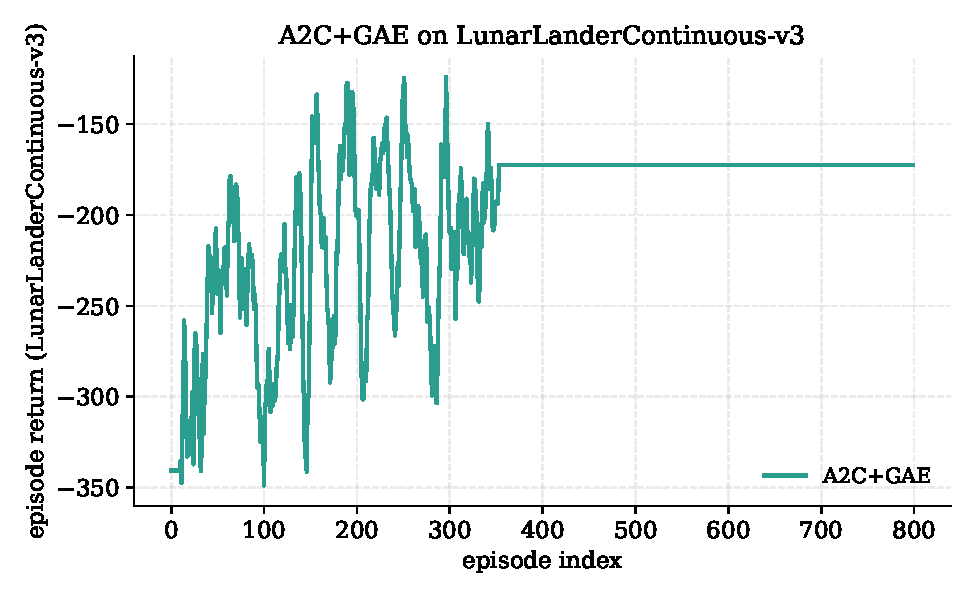
\includegraphics[width=0.85\linewidth]{figs/a2c_lander.pdf}
\caption{LunarLander-Continuous training curve. Synchronous A2C+GAE ($N=8$ vector envs, $T_R=128$) reaches positive returns within $\sim$200 updates. Mean and IQR over 3 seeds.}
\label{fig:a2c-lander}
\end{figure}

\begin{figure}[h]
\centering
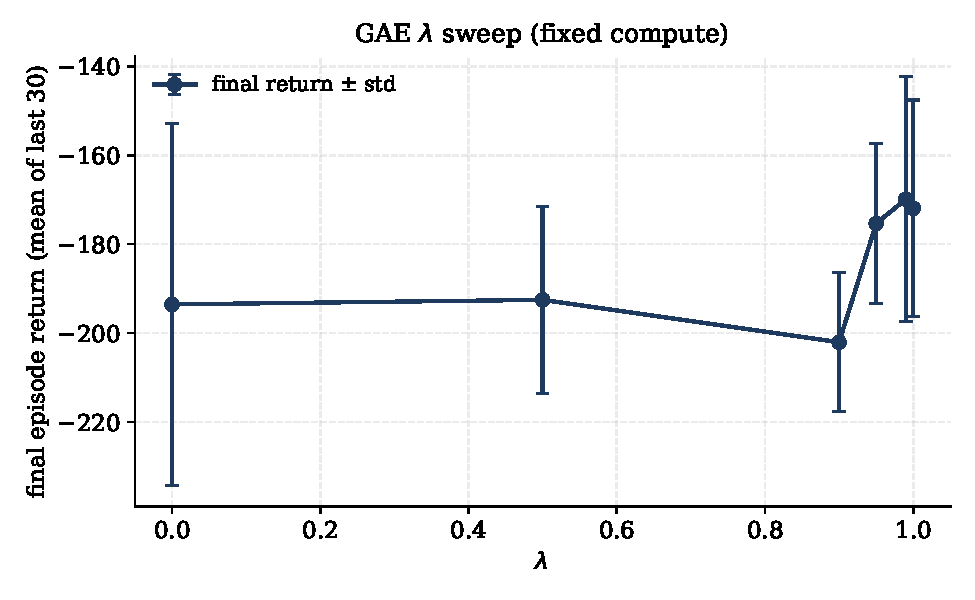
\includegraphics[width=0.85\linewidth]{figs/lambda_sweep.pdf}
\caption{GAE bias--variance sweep. Final return after a fixed compute budget as a function of $\lambda \in \{0.0, 0.5, 0.9, 0.95, 0.99, 1.0\}$.}
\label{fig:lambda-sweep}
\end{figure}

\chapter{Safety angle}

\begin{safetyangle}
The KL trust-region in TRPO is not just an optimisation gadget --- it is \emph{the structural safety mechanism} of modern policy methods.

\paragraph{Why KL is the right safety knob.}
Total variation between a policy and a reference policy is exactly the maximum-over-events probability that they behave differently. Pinsker's inequality, $\TV(p,q) \le \sqrt{\tfrac12 \KL(p\|q)}$, makes a small KL imply a small worst-case behavioural divergence. For a high-stakes RL deployment, ``my new policy differs from the old reviewed-and-approved one by at most $\sqrt{\delta/2}$ in any event probability'' is a meaningful guarantee.

\paragraph{The pattern reappears everywhere downstream.}
\begin{itemize}[leftmargin=*]
  \item RLHF/PPO for LLMs: penalty $-\beta \KL(\Policy_\theta \| \Policy_\text{ref})$ keeps the policy near the SFT model and is the only thing standing between the agent and reward-hacking the reward model (Stiennon et al.\ 2020, Ouyang et al.\ 2022).
  \item DPO and friends (week 19): the closed-form $r(x,y) = \beta \log \Policy/\Policy_\text{ref}$ \emph{is} the KL constraint, made explicit.
  \item Constrained RL (week 16): CPO is TRPO with an extra cost-constraint solved jointly via a closed-form 2D quadratic.
\end{itemize}

\paragraph{Failure modes.}
\begin{enumerate}[leftmargin=*]
  \item \emph{Damping mis-set.} A too-small CG damping causes the Fisher matrix to be effectively singular along low-variance directions and the line search collapses. Mitigation: set damping to $10^{-2} \cdot \mathrm{trace}(F)/|\theta|$ as a sane prior.
  \item \emph{KL divergence asymmetry.} TRPO penalises $\KL(\Policy_\text{old}\|\Policy_\text{new})$, not the reverse. This is mode-covering, not mode-seeking; in a multi-modal optimal policy you may end up in the wrong mode but with a reassuring small KL.
  \item \emph{Stale advantages on long-running envs.} If $\Vfn_\phi$ has not converged, $\hat\Adv$ is biased and the trust region protects a wrong direction. Schulman 2015 fits $\Vfn_\phi$ to convergence with L-BFGS every outer iteration to avoid exactly this.
\end{enumerate}
\end{safetyangle}

\chapter{Matching application}

\begin{matching}
\textbf{Trust regions for production policy updates in synthetic insurance.}

Imagine the current synthetic insurance lead-router has been A/B-tested and shipped --- a known-quality policy $\Policy_\text{old}$. We want to fine-tune it with the latest week of logged conversions, but with a hard guarantee that the new policy is behaviourally close to the old one (so the existing SLA, audit trail, and broker-fairness review remain valid).

\paragraph{Direct translation.}
\begin{itemize}
  \item \textbf{Surrogate $L$:} importance-weighted conversion reward, $\E_{s,a\sim\Policy_\text{old}}[(\Policy_\theta/\Policy_\text{old}) \cdot \Adv]$, where $\Adv$ is fitted from the logs.
  \item \textbf{Trust region:} $\bar{\KL}(\Policy_\text{old} \| \Policy_\theta) \le \delta \approx 10^{-3}$. This bounds the maximum change in any broker's expected slot-share to $\sqrt{\delta/2} \approx 2\%$ --- a reasonable per-week ceiling for a regulated marketplace.
  \item \textbf{Solver:} A2C+GAE plus a back-tracking line-search against the empirical KL is sufficient; we do not need the full conjugate-gradient TRPO machinery for the modest-sized policies in production.
\end{itemize}

\paragraph{synthetic ATS connection.}
For candidate-to-role matching the same architecture buys a different guarantee: ``no candidate's expected interview probability changes by more than $\eta$ between weekly model retrains.'' This is exactly what compliance teams demand from ML systems with disparate-impact reviews; the KL trust region is the math that lets you offer it.
\end{matching}

\chapter{Exercises}

\begin{enumerate}[label={},leftmargin=0pt,labelsep=0pt]
  \item \textbf{E1} ($\star$) Prove identity $(\dag)$.
  \item \textbf{E2} ($\star$) Implement \texttt{compute\_gae} and unit-test against the MC limit.
  \item \textbf{E3} ($\star\star$) Show GAE at $\lambda=0$ equals one-step TD; at $\lambda=1$ equals MC.
  \item \textbf{E4} ($\star\star$) Train A2C+GAE on LunarLander-Continuous.
  \item \textbf{E5} ($\star\star$) Sweep $\lambda$; reproduce Figure~\ref{fig:lambda-sweep}.
  \item \textbf{E6} ($\star\star$) Derive the Fisher matrix for a diagonal Gaussian policy.
  \item \textbf{E7} ($\star\star\star$) Code a conjugate-gradient solver and verify $F^{-1}g$ on a toy MVN.
  \item \textbf{E8} ($\star\star\star$, meaningful objective) Trust-region weekly retrain on logged matching data; show KL bound implies bounded slot-share change.
\end{enumerate}

\chapter{Further reading}

See \texttt{extended\_reading.pdf}. Five papers: Mnih et al.\ 2016 (A3C), Schulman et al.\ 2015 (GAE), Kakade 2001 (NPG), Schulman et al.\ 2015 (TRPO), Engstrom et al.\ 2020 (Implementation Matters). Sourced from \texttt{research/deeprl\_core\_sota.md} \S 2.2--2.5.

\end{document}
